\chapter{Expanção em uma dimensão}
 Definido o método dos elementos finitos com a formulação de Galerkin, temos diferentes meios para resolver o problema. Anteriormente resolvemos uma equação diferencial usando elementos finitos com \textbf{equações lineares}. Discretizando o espaço em elementos de tamanho \textbf{h} e utilizando as técnicas de derivação e integração numérica utilizando polinômios de grau \textbf{p}, podemos utilizar a combinação desses métodos nos fornece aproximações com erros menores, para diferentes métodos.
 O método \textbf{p} utiliza um problema com um número de elementos fixo e para cada elemento usamos um  polinômio de grau \textbf{p} e verificamos a convergência do erro para cada grau desse polinômio. Temos o método \textbf{h} no qual fixamos o grau do polinômio e aumentamos o número de elementos, diminuindo o tamanho \textbf{h} de cada elemento.
 E o método espectral \textbf{hp} é a combinação de ambos os métodos anteriores, onde variamos o tamanho do elemento e o grau do polinômio para verificar a convergência do erro. 
 \section{Método h}
 Utilizamos esse método nos permite resolver problemas de geometrias convexas, no caso em uma dimensão, o problema nos permite resolver problemas com singularidades. Podemos verificar esse fenômeno com a própria função de Runge anteriormente:
\begin{figure}[!h]
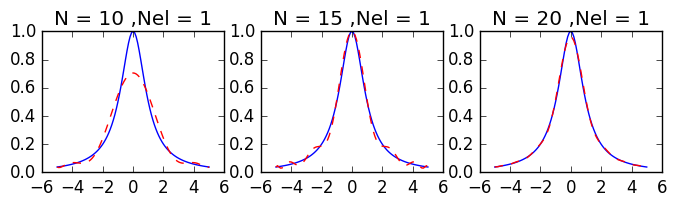
\includegraphics[width=0.7\textwidth, center ]{figuras/compara_metodo_n.png}
\caption{polinômio base de Lagrange para N  pontos em apenas um elemento}
\end{figure}
\\ Vimos que a aproximação acontece para um polinômio de grau elevado, no caso anterior, n igual a 20. Porém  aumentando o número de elementos e tendo fixo o grau do polinômio, vemos que essa singularidade é contornada.


 
